\subsection{Uncertain Graph Application Measures}
\begin{figure}[!htb]
    \centering
    \subfigure[PPI]{
    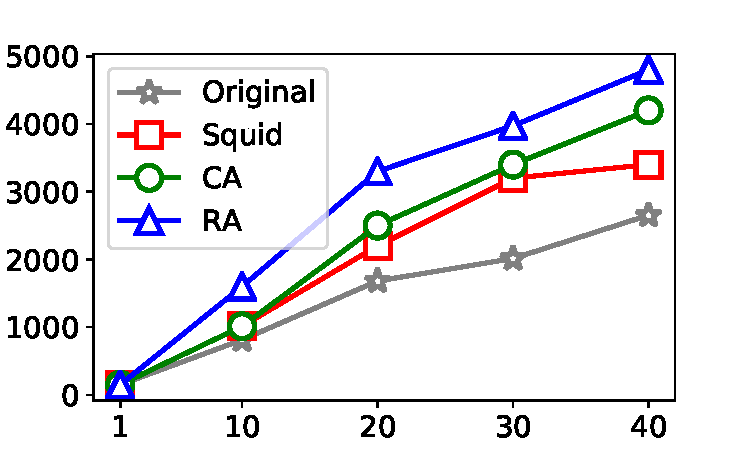
\includegraphics[height=4cm]{expResult/ppi_IM.pdf}
    }
    \subfigure[BK]{
    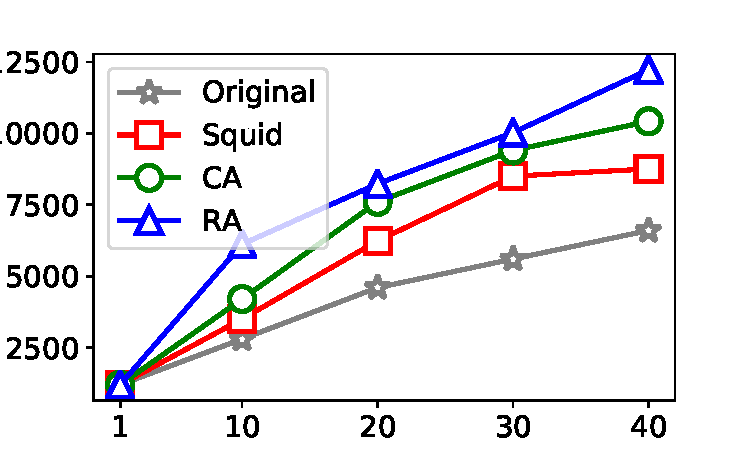
\includegraphics[height=4cm]{expResult/bk_IM.pdf}
    }
    \caption{ Results of the influence maximization algorithm on PPI and BK datasets, compared to sanitized outputs where $k$=100.}
    \vspace{-15pt}
    \label{fig:IM}
\end{figure} 
For a sanitized graph to be meaningful for research use, it should produce 
the close results as the original graph in the application-level settings. 
Influence Maximization is known as essential techniques with advertisement and public relation campaigns.
It tries to locate users in the network who can most quickly spread information through the network. 
Usually, related algorithms start with identifying the nodes which can maximize influence and model the spread of influence through network how many users has ultimately reached.  
Motivated by these facts, we compare the result of influence maximization on sanitized outputs and original graphs. 
In general, it enables us to quantify the trade-off between application utility and privacy protection. 

\textbf{Methodology.}~We used the sampling method to get the expectation value of influence. For each sampled graph, we adopt the degree discount method (a heuristic-based method with light computation) to find the most influential nodes (seeds) on a deterministic graph. Starting from those seeds, we run the weighted cascade influence dissemination model to determine the number of reached users in the network. 

For the limit of computation resource (memory overhead), we only perform the set of experiment over PPI and BK datasets. We report the expected number of reached nodes when the number of initial seeds in Figure~\ref{fig:IM}. 
There are clear and visible trends across PPI and BK datasets. 
Graphs with privacy protection diverge from the results of original graphs.
We found that our method excelled in preserving the information propagation pattern, followed by CA that aim explicitly at preserving linear property.  
Overall, our experimental assessment on influence maximization applications confirms our intuition: by incorporating the possible world semantics into the core of anonymization such as edge selection and uncertainty injecting, one can achieve the same desired level of anonymity with a smaller impact in the uncertain graph utility.  